\documentclass[11pt,letterpaper]{article}

%%% PACKAGES
\usepackage[utf8]{inputenc}
\usepackage{microtype}
\usepackage[T1]{fontenc}
\usepackage{lmodern}
\usepackage{booktabs}
\usepackage{color}
\usepackage{colortbl}
\usepackage{graphicx}
\usepackage{epstopdf}
\usepackage{epsfig}
\setlength{\parindent}{0cm}
\usepackage{multirow}
\usepackage{enumerate}
\usepackage{longtable}
\usepackage{listings}
\usepackage[table]{xcolor}
\usepackage{amsmath}
\usepackage{amsfonts}
\usepackage{amssymb}
\usepackage{float}
\usepackage{times}
\usepackage{multicol}
\usepackage{geometry}
\usepackage{wasysym}
\usepackage{wrapfig}
\usepackage{amsbsy}
\usepackage{flushend}
\usepackage{url}
\usepackage[percent]{overpic}
\usepackage{caption} 
\usepackage{pgfplots}
\usepackage{sectsty}
\usepackage[all]{nowidow}
\usepackage{tikz}
\usetikzlibrary{er,positioning,bayesnet}

%%% BIBLIOGRAPHY
% \usepackage[hidelinks]{hyperref}
\usepackage[backend=biber,date=short, style=apa]{biblatex}
\addbibresource{Bibliografia.bib}

%%% PAGE DIMENSIONS
\geometry{top=3cm, bottom=2.5cm, left=2.5cm, right=2.5cm}

%%% DATE
\usepackage{datetime}
\newdateformat{monthyeardate}{%
\monthname[\THEMONTH], \THEYEAR}

%%% LINE SPACING
\renewcommand{\baselinestretch}{1}


\begin{document}

%%%% TITLE PAGE
\begin{titlepage}
    \begin{figure}[H]
    \centering
    \vspace{-1.2cm}
    \includegraphics[scale=0.55]{Imagenes/logo_universidad.png}
    \end{figure}
    \vspace{1cm}
    
    \begin{center}
    Departamento de Obras Civiles\\
    \vspace{4cm}
    
    {\Large \textbf{WIND-EFFECTS ON BAR-BUILT ESTUARY HYDRODYNAMICS }}\\
    \vspace{2cm}
    {Memoria de Título presentada por}
    \vspace{0.5cm}
    
    {\Large{\textbf{Dhannai Tamara Sepúlveda González}}} \\
    \vspace{1.5cm}
    
    {como requisito parcial para optar al título de la carrera de}\\
    \vspace{0.5cm}
    
    \textbf{Ingeniería Civil}\\
    \vspace{1.5cm}
    
    {y el grado de}\\
    \vspace{0.5cm}
    
    \textbf{Magíster en Ciencias de la Ingeniería Civil}
    
    \vfill
    {Profesor Guía}\\
    {Megan Elizabeth Williams}\\
    \vspace{0.5cm}
    \textsc{\monthyeardate\today}\\
    \end{center}
    
    \clearpage
    \parindent=0mm
    \end{titlepage}
    
    %%HOJA DE FIRMAS%%
    \begin{titlepage}
    \begin{figure}[H]
    \vspace{-1cm}
    \includegraphics[scale=0.45]{Imagenes/logo_universidad_letras_lateral.png}
    \end{figure}
    
    \vspace{2.5cm}
    
    \noindent{\Large \sc{TÍTULO DE LA TESIS:}}\\
    \vspace{0.3cm}
    
    \noindent{\Large \textbf{WIND-EFFECTS ON A BAR-BUILT ESTUARY HYDRODYNAMICS }}\\
    \vspace{1.5cm}
    
    \noindent{\Large \sc{AUTOR:}}\\
    \vspace{0.3cm}
    
    \noindent{\Large \textbf{DHANNAI TAMARA SEPÚLVEDA GONZÁLEZ}}\\
    \vspace{2cm}
    
    \noindent{TRABAJO DE MEMORIA, presentado como requisito parcial para optar al grado de MAGÍSTER EN CIENCIAS DE LA INGENIERIA CIVIL de la Universidad Técnica Federico Santa María.}\\
    \vspace{1.5cm}
    
    \noindent{\Large{Nombre Profesor Guía:\hspace{3.5cm}  Megan Williams}}
    \vspace{1.5cm}
    
    \noindent{\Large{Nombre Miembro 1 Comisión:\hspace{2cm}  .............................................................}}
    \vspace{1.5cm}
    
    \noindent{\Large{Nombre Miembro 2 Comisión:\hspace{2cm}  .............................................................}}
    \vspace{1.5cm}
    
    \vfill
    \begin{flushright}
        {Valparaíso, Chile, September, 2022}\\
    \end{flushright}
    \end{titlepage}
    
    \clearpage
    
    
    %%% DOCUMENT
    \newpage
    \begin{center}
        \textsc{\textbf{\Large Wind-effects on bar-built estuary hydrodynamics}}
    \end{center}
    Dhannai Sepúlveda$^1$, Megan Williams$^1$\\
    
    1 Universidad Técnica Federico Santa María\\
    
    \textbf{Abstract}\\
    Although bar-built estuaries are widespread on Mediterranean coasts all around the world, including central Chile, little research has been undertaken on its closed state, when its system is transformed into a salty lagoon. Understanding the dependence of hydrodynamic response and thermohaline-stratification on strong wind events and its associated transport and mixing is of prime importance on the impact of water quality and eutrophication on ecosystems in coastal lagoons. In this study, we analyze the role of external factors such as wind velocities, freshwater flow, and wave overtopping in the hydrodynamics of a shallow, highly salt-stratified bar-built estuary. Vertical mixing and forcing currents, governed by wind surface stress, were quantified for diurnal and hourly time scales.
    
    Data collected in early 2012 at Pescadero Estuary, California shows that in a close state there is a strong stratification and strong wind events during its closed state and due to its morphology wind is channelized into the along-estuary direction, causing the lagoon to receive mainly local forcing. Frequency spectral analysis is used to identify seiches on the surface due to upwelling caused by the wind. Wavelet analysis was also used to identify wave overtopping on the sand bar and observe the real effect of saline water entering the estuary. 
    
    During strong wind events, buoyancy frequency was reduced to almost 0 from the 0.1 $s^{-2}$ that the estuary usually had, and in some cases not return to its original value, showing upwelling and mixing of the water column. However, these effects varied over time depending on water level due to constant inflow from Pescadero and Butano creek. Some indicators like potential anomaly showed a good correlation with wind stress during the studied period. These preliminary findings show that wind effects are dominant in forcing vertical exchange of layers and generating currents at Pescadero.\\
    
    \textit{Key words: bar-built estuaries, wind stress, stratification, upwelling, mixing}

    \newpage
    \section*{ACKNOWLEDGEMENTS}
    
    klsdklsdklsd
    \newpage
    
    \tableofcontents
    
    \listoffigures
    
    \listoftables
    
    \newpage
    
    \section{Introduction}
    
    
    By the definition of \citeauthor{mcsweeney2017intermittently} (\cite*{mcsweeney2017intermittently}) estuaries are "geomorphic systems which represent the transition between fluvial and marine environments". These coastal waterbodies such as fjords, bar-built estuaries, and coastal lagoons are constantly exposed to anthropogenic or natural disturbances due to their productive importance (\cite{schernewski2002baltic, martinez2007coasts}) and global changes (\cite{grez2020evidence}). These ecosystems are exposed to sea-level rise, changing precipitation, and temperature patterns, in addition to a growing human population that is largely concentrated near the coast (\cite{neumann2015future}). This type of habitat is highly variable and dynamic and is where complex physical and biochemical processes take place.\\
    
    Bar-Built estuaries are systems characterized by periodic/intermittently inlet closure through a sand bar (\cite{whitfield2007review}). These are mainly found in Mediterranean climates such as Chile, California, South Africa, and Australia (\cite{mcsweeney2017intermittently}). Closure occurs when a sand berm forms in the entrance channel and it can occur both seasonally or irregularly throughout the year (\cite{Behrens2013}). However, it is common that annual variability dominates closure events due to the marked seasonal cycles for rain and river flow observed in this type of climate (\cite{Ranasinghe2003}). Despite the variable nature of these systems, they are vital for many species that have adapted to take advantage of the closed-mouth condition (\cite{viaroli2008community}).\\
    
    When the estuary inlet closes, external factors like wind, river flow, and wave overtopping can impact its structure. This could be causing changes in the density due to fresh and saltwater input or surface stress by wind effects, causing upwelling, mixing, or circulation changing the estuarine ecosystem (\cite{Ranasinghe1999}).  The wind is the main external factor present, but the stratification makes it difficult to energize the denser layer, leading in some cases to a suppression of the turbulence under the pycnocline (\cite{Cousins2010}). The foregoing makes these systems highly dynamic due to their variability in temperature and salinity, where complex physical and biogeochemical processes of oceanic and freshwater environments interact. Species that inhabit these types of environments are vulnerable to conditions such as hypoxia or anoxia in the lower layers (\cite{Kelly2018}) or the retention of nutrients in the bottom (\cite{Cousins2010}) and when there is upwelling or mixing it could happen abrupt changes for marine life and generate them some problems or even death (\cite{marti2008relating}).\\
    
    Previous research shows the response of the shear stress produced by the wind in large thermal-stratified lakes (\cite{Coman2012, Laval2008, avalos2019natural}), where it was observed how the wind stress affects these waterbodies when they have frequencies close to their natural oscillations and how the upwelling events caused by it cause variability in temperature. Even so, there is limited information on the hydrodynamic effects of the wind in small and saline-stratified lagoons, which would be interesting to study to learn how the wind affects their behavior and structure.\\
    
    Currently, this type of estuaries is widely spread in Chile, because their seasonal conditions are similar to those of other places, already mentioned, where they are found, and despite this, there are few studies carried out in the country on the subject. In \citeauthor{dussaillant2009} (2009) an investigation was carried out on the Yali reserve, one of the most important wetlands in the central zone of Chile, whose knowledge must be complemented to fully understand the small and highly stratified coastal systems.\\
    
    \subsection{The Pescadero estuary}

Pescadero Estuary is a small and highly stratified bar-built estuary located at the confluence of Pescadero Creek and Butano Creek on the California coast. It is located 60 [km] south of San Francisco Bay and 40 [km] north of Monterrey Bay (Fig. \ref{fig:locPDO}). The Mediterranean hydroclimate of Pescadero is characterized by an average annual rainfall of 750 [mm] with a cooler and more pronounced wet season that extends from November to April and a warmer dry season from May to October  (\cite{climatedata2021}).\\

\begin{figure}[h!]
    \centering
    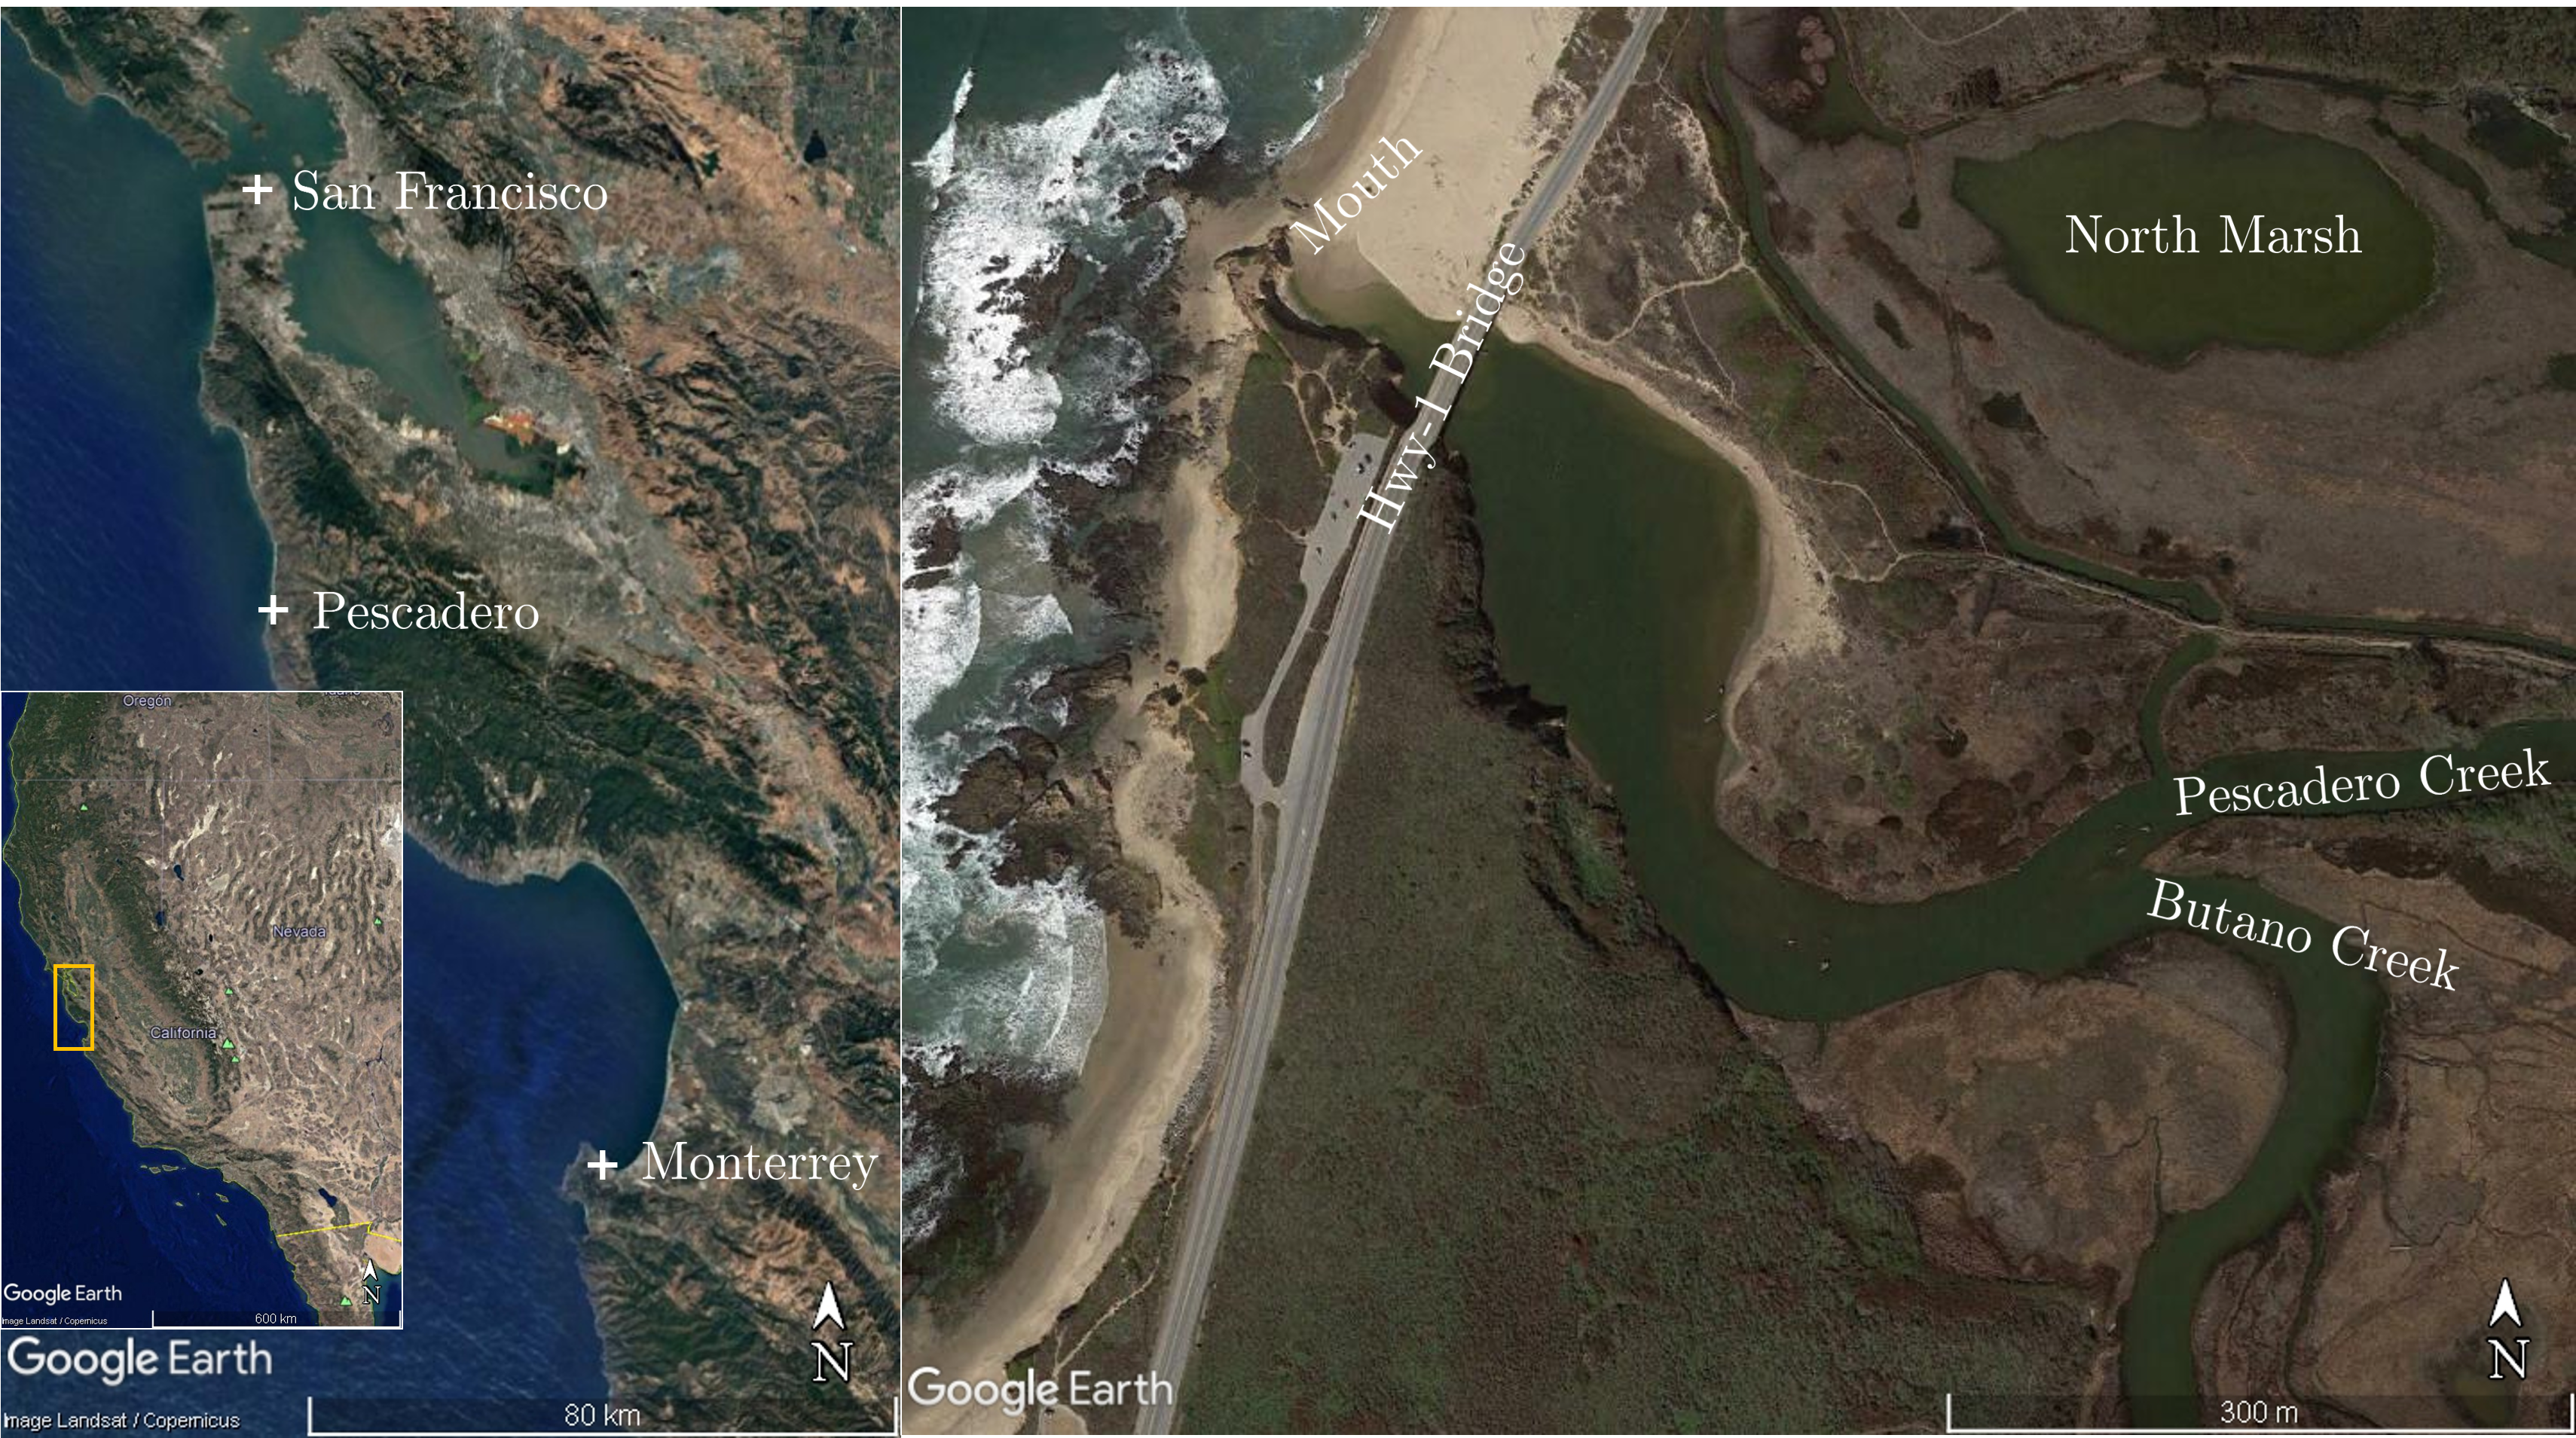
\includegraphics[scale=0.6]{Imagenes/mapa1.png}
    \caption{Location of Pescadero Estuary on California's Coastline. Images reprocessed from Google Earth.}
    \label{fig:locPDO}
\end{figure}

The sand barrier placed at the inlet of Pescadero closes the estuary from the sea, changing its behavior to a stratified lagoon which usually happens during the dry season (\cite{Williams2014}). Inlet rupture usually occurs during the wet season when precipitation increases flow and the lagoon fills to overflowing, leading to the scour of a new channel between the lagoon and the return of tidal action and seawater intrusions to the estuary (\cite{largier2015}). During periods when the mouth of the estuary is closed, the water level of the lagoon rises and could flood the surrounding marshy land. \\

The significance of this site lies in the detection of fish kills after the breaching of the lagoon mouth after an extended closure (\cite{largier2015}). Also, there are agricultural lands on the surroundings that have a productive importance for the local community in addition to other concerns as winter flooding of low-lying lands, in which exists some roads and parts of the town, or the presence of a wide diversity of habitats and microhabitats in the estuary.\\

Pescadero has two main water inputs: freshwater inflow and saline water, which sometimes get mixed and other times form a two-layer structure. The behavior of the estuary depends on the mouth state, where we can observe an 'open' and 'closed' state. Pescadero receives freshwater inflow from two relatively small watersheds, which have a highly variable discharge, following precipitation that varies from day to day through the wet season, as well as seasonally and between years (\cite{largier2015}). The Pescadero watershed is about twice the size of the Butano watershed, and produces 57\% of the streamflow (\cite{Williams2014}). On the other hand the Northern Californian coast experiences a semidiurnal tide with a neap tide range of under 1 m and a spring tide range up to almost 3 m (\cite{Williams2014}). Saltwater get into the estuary easily during open state, but when the inlet is closed seawater has to overtop the sandbar to get into the estuary, which happens occasionally during high tide and strong waves.\\

When the mouth is closed the estuary takes a stratified structure fed by the freshwater input and the sporadic wave overtopping saline water. In this form is more difficult to energize the water column, but it can happen with external factors as wind stress in the surface or from the discharge and the wave overtopping. However, vertical transport in Pescadero couldn't be from density-driven exchange, because the estuary would be always saltier than the creeks input water, so it always will stay on the top of the water column making the estuary stratified. Even that, in Pescadero there is a light density/salinity gradient due to the freshwater input upstream and the saltwater overtopping the bar at the other end.\\

\subsection{Motivation}

In its state of disconnection from the ocean (i.e., closed state), the estuary can take the form of a shallow stratified lagoon, due to the presence of saltwater and freshwater from fluvial inputs (\cite{Behrens2016}). This estuary state could lead to eutrophication if there are no energy inputs to the system (\cite{nunes2014responses}), and usually, the wind is the main source, driving to mixing and destratification in small bar-built estuaries (\cite{Gale2006}) triggering processes that impact mixing and circulation, which could affect the marine life of the estuary (\cite{marti2008relating}). \\

As said before, the wind is the principal driver of mixing present, but sometimes stratification makes difficult to energize the denser layer, leading in some cases to suppression of turbulence below the pycnocline (\cite{Cousins2010}). This could cause hypoxia or anoxia in the lower layers (\cite{Kelly2018}) or retention of nutrients in the bottom (\cite{Cousins2010}) and when there is upwelling or mixing, abrupt changes could occur for marine life and generate problems or even death (\cite{marti2008relating}).\\  

Due to the latter, these waterbodies are highly dynamic, and this makes them sites of great importance for research. On the other hand, estuaries are the connection between the earth and the ocean, receiving waters coming from rivers and creeks that are exposed to anthropogenic effects, causing changes in freshwater flow or temperature, in addition, to being subjected to sea level rise and wave climate variations (\cite{grez2020evidence, holt2010potential, thorne2021wetlands}). Besides, in the estuaries, of their contact with the coast and rivers, activities such as fish farming or agriculture are developed, so they have economic and social importance to communities. \\

The response to strong and sustained wind stress in a closed state bar-built estuary starts with a setup of the surface and a change in the pressure gradient. This will cause the pycnocline to tilt upwards at the upwind end of the estuary leading sometimes the bottom layers to rise to the surface. The reduction or end of this wind forcing releases the pycnocline from its tilted position and return to horizontal. The upwelling effect caused by wind forcing has potential relevance in nutrient and oxygen exchange between layers (\cite{Kelly2018}) and has been studied widely in lakes using temperature measurements (\cite{Coman2012, delafuente2010strong, roberts2021setup}), however, there are fewer studies that observe this kind of behavior at bar-built estuaries or in smaller coastal lagoons. \\

\section{Objectives}

\subsection{General objective}

The mean goal of the present work is to study velocity and density variability in the water column of a small and highly stratified estuary during its closed state and relate them to wind stress, to use the collected information to delve into the study of water bodies of this type. In addition, this research seeks to gain a better understanding of the relationship between wind stress and the behavior of layers of different densities within the closed state estuary.  Our case study is the Pescadero Estuary, a bar-built estuary in California that represents many other small inlet systems elsewhere in the world. Data sets of wind and pressure at this site containing several mouth openings and closures are going to be used.\\

\subsection{Specific objectives}

The specific objectives of this study are:
\begin{enumerate}
    \item [(1)] To make a time-series analysis of data collected from the Pescadero estuary using depth, temperature, salinity, and velocities collected from the estuary and the wind velocities obtained at 3 meters height.
    \item [(2)] To determine the effect of wind stress on the hydrodynamic characteristics of the estuary while the inlet is closed focusing on stratification.
    \item [(3)] To study the wind-estuary interaction and the effects of other external factors such as water inflow and wave overtopping in this interaction.
\end{enumerate}

\section{Literature review}

\subsection{Bar-built estuaries in the ecosystem and the community}

Climate change is affecting multiple marine ecosystems globally (\cite{hewitt2016multiple}). Its been detected that the global oceanic oxygen content has decreased during the last five decades \cite{schmidtko2017decline} and that air temperature is increasing in oceans (\cite{omstedt2004baltic, jones1999surface}) which according to models can affect stratification in northwest European continental shelf and Baltic Sea due to a decrease of salinity at the surface (\cite{hordoir2012effect, holt2010potential}) changing the number of days that stratification is present causing impact in nutrient flux. Also, some studies expect that the absolute mean sea level on Chilean coasts rises between 0.35 to 0.74 m in the next 80 years (\cite{winckler2020evidence}). The effects of climate change can put at risk the coastal zones, including estuaries and coastal lagoons which are especially abundant ecosystems in flora and fauna.\\

In addition, there is evidence that there is a decrease in surface wind speeds in Northern Europe (\cite{woolway2017atmospheric}) and an increase in along-shore winds in the Chilean coastal zone (\cite{winckler2020evidence}). It is known that changes in surface wind speed affect the number of days that a lake is stratified, which affects the nutrient availability and quality of a waterbody, changing the amount of oxygen present in deep waters (\cite{woolway2017atmospheric}). It is important to study wind effects in estuaries to be able to quantify how wind-speed changes will affect these environments.\\

In central Chile, there is a decrease in river discharges affecting buoyancy and stratification (\cite{winckler2020evidence}), which can be causing a wide range of changes in estuarine and marine ecosystems, including changes in oxygen availability. These changes can impact fish populations and other autotrophic organisms.\\

The importance of intermittently closed estuaries goes beyond local impacts. These estuaries can accumulate sediment and minerals while the inlet is closed (\cite{thorne2021wetlands}), and in rainy seasons they open the mouth naturally because of the increase in freshwater inflow (\cite{hoeksema2018factors}). This process settles sediments to the near marshes helping to maintain their elevation according to the sea level, mitigating the consequences of sea level rise (\cite{thorne2021wetlands}). On the other hand, it is very common opening the mouth artificially to avoid flooding the near lands (\cite{Behrens2013}) which doesn't allow the sediments to set correctly in the marsh platform  (\cite{thorne2021wetlands}). ENSO (El Niño Southern Oscillation) is the principal cause of the opening and closure of the mouth (\cite{mcsweeney2017intermittently}), but this phenomenon can change its occurrence in the next years, affecting estuaries' dynamics and water quality all around the world (\cite{thorne2021wetlands}).\\

Climate change is affecting bar-built estuaries' dynamics and water quality. Increasing river discharge due to more precipitation could lead to increase erosion and the number of suspended particles of sediment in the water. Enhanced sediment concentration could lead to accumulation in the estuary making the inlet close, changing the equilibrium of opened and closed state of the sand bar, which along with the increase of freshwater input could flood the surrounding land (\cite{peeters2009currents}). Consequently, depending on the vegetation present and its oxygen demand, deep-water oxygen may be reduced or suppressed (\cite{Kelly2018}, \cite{Largier2021}). Also, the density of the surface waters will be reduced and thus could change the estuary behavior to external factors such as wind stress. \\

On the other hand, bar-built estuaries are under continuous anthropogenic stress due to their closeness to human settlements (\cite{clark2019systematic}) and their productive importance. Dams constructed upstream for water storage reduce the freshwater that goes to the ocean, causing the retention of suspended sediments. This results in a change in the morphology of the estuary due to not receiving the sediments that used to accumulate in the inlet, leading to premature scour of the sand bar (\cite{peeters2009currents}). Also, to prevent the flood of roads or agricultural lands that settle nearby, the community plan the opening of the inlet artificially, which could result on abrupt changes on the estuary ecosystem (\cite{Behrens2013}). \\

\subsection{How bar-built estuaries are studied in Chile and around the world}

There are plenty of methods and instrumental techniques to measure the behavior of estuaries and lakes at a small scale (\cite{Wuest2003}), methods that can be used with new data and get improved for future works and be more specific for the different types of waterbodies. \citeauthor{mcsweeney2017intermittently} (\cite*{mcsweeney2017intermittently}) studied the bar-built estuaries all around the world and their climatic, marine, and fluvial conditions to classify them and quantify the drivers of their distribution in each continent. That can "allow predictions of estuary response to climate change and human impacts to be made and to ultimately assist with integrated coastal management into the future".\\

\citeauthor{dussaillant2009} (\cite*{dussaillant2009}) studied a Chilean coastal lagoon in its open and closed state and observed that in its closed state the rainfall influence was not important except for the storms that open the inlet to the sea. He also observed that wind is very important in water level fluctuations in the disconnected phase. He studied the connected phase using a general pattern, spectral, and Fourier analysis.\\

\citeauthor{Kelly2018} (\cite*{Kelly2018}) observed that in stratified waterbodies, when the vertical exchange is limited, it can be oxygen depletion present, causing hypoxia and anoxia, a factor that is related to fish kills in Pescadero (\cite{largier2015}). \citeauthor{Kelly2018} proposed that tidal influence oxygenated the deeper layers in a saline lagoon in some specific events and observed that the same conditions were present when there was wind-driven upwelling, showing a relation between tidal influence and wind stress in vertical mixing.\\

\citeauthor{Behrens2016} (\cite*{Behrens2016}) observed the salt intrusion in a bar-built estuary and its differences between closed and open state conditions. The study found the presence of alternating shallow sills and deep pools, which act to trap the salt after intrusion, and suggested that internal seiche motions in the outer estuary initiate the intrusion by lifting saline water in the pycnocline high enough to crest the sills. This salinity intrusion extends to distances of several kilometers from the beach.\\

Studies carried out in Rodeo Lagoon (\cite{Cousins2010}), a shallow strongly-stratified lagoon, found that stratification by brackish water leads to a pronounced suppression of turbulence below the pycnocline and confines nutrients released from the sediment into the lower layer. Those can be confined for up to several months, compared to the rapidly flushed overlying fresh layer. They observed that in the lagoon wind is the dominant source of mixing because of a lack of other energy inputs and destratification by wind mixing allows for the redistribution of nutrients from the bottom brackish layer.\\

\subsection{Pescadero estuary studies}

Pescadero estuary has literature related to management plans focusing on productivity (\cite{curry1985pescadero}) or in preserve the hydrology of the estuary (\cite{williams1990pescadero}. But recent studies have been motivated on the fish kills that have been observed in the last years, signaling that when the sandbar closes stratification leads to the creation of an anaerobic environment in bottom waters (\cite{sloan2006ecological}). Also, geochemical analysis to sediments showed that the transition from closed to open state leads to poor water conditions within the Pescadero Estuary, with many indicators reaching values that are outside the range of optimal conditions for fish or aquatic life (\cite{richards2018}). \\

In addition, it has been studied more physical phenomena like the effects of the constriction that generates the mouth in its open state, showing a discontinuous tidal forcing in the estuary (\cite{williams2016}). \citeauthor{williams2016} observed that wave setup and tides set the estuarine water level, while the mouth sandbar limits ocean gravity waves to enter the estuary but permits infragravity motions to pass through the inlet, which induced energetically important high velocities, highlighting the strong dependence of hydrodynamics of small bar-built estuaries on nearshore processes. Also, hydrodynamic processes in Pescadero are comparable to similar estuaries along the western coast of the Americas as well as in Australia, South Africa, and in estuaries in Mediterranean climates on the Atlantic west coast of Europe, as well as in shallow sandy inlets elsewhere.\\

\section{Methods}

\subsection{Field observations}

Four field campaigns were carried out between 2010 and 2012 described in the work of \citeauthor{Williams2014} (\cite*{Williams2014}) and \citeauthor{williams2016} (\cite*{williams2016}), but in this work, we will focus exclusively on the data between January and March 2012 to analyze the behavior of the estuary in a closed state. Measurements were made using instruments for speed and depth, as well as including a meteorological station to collect wind speed and direction data. Depth data were collected using moored pressure, conductivity, and temperature sensors (CTD) placed at different heights and distributed along the estuary at four points as shown in (Fig. \ref{fig:mapPDO}), called Near Mouth (NM), Mid-Lagoon (ML), Deep Channel (DC), and Pescadero Creek (PC). Density profiles were made on February 16th with a CTD logger around 5 p.m. when the wind was calm at the locations indicated in (Fig. \ref{fig:mapPDO}).


\begin{figure}[h!]
    \centering
    \includegraphics[scale=0.6]{Imagenes/mapa2.png}
    \caption{Pescadero estuary map and location of the sensors (NM: Near Mouth, ML: Mid-Lagoon, DC: Deep Channel and, PC: Pescadero Creek), instant profiles, and meteorological station. }
    \label{fig:mapPDO}
\end{figure}

Velocity measurements were made with an Acoustic Doppler Current Profiler (ADCP) anchored to the bottom of the estuary at location DC. This instrument is designed to be used in deeper water, so data collected from the surface could be affected by the interference caused by reflection. Due to the latter, the data were removed from the record. On the other hand, the ADCP has a blank space before measuring speed, so the first measured point was 71 cm above the ground, meaning there is only a window of velocity data in the water column. \\

For wind speed data, an anemometer was installed 3 m above the water level in marshy land adjacent to the estuary (Fig. \ref{fig:mapPDO}). It was observed that due to the topography of the sector, the wind direction is channelized along the estuary, so the directions between 300 and 360 degrees come from the ocean and the wind that blows from 100 to 170 degrees comes from inland.\\

To complete the information, the freshwater streamflow into the Pescadero estuary is estimated based on a United States Geological Survey (USGS) gauge located on Pescadero Creek 8.5 km upstream from the mouth of the estuary (USGS 11162500). The tide height data in San Francisco Bay and Monterrey Bay (stations 9414290 and 9413450 respectively) were obtained from the National Oceanographic and Atmospheric Administration (NOAA) and waves data were obtained from the National Data Buoy Center, 40 km in the ocean from the coast of Half Moon Bay (station 46012). Additionally, the bottom pressure measurements at each sensor were corrected for sea-level atmospheric pressure measured at the nearest weather station located at the Half Moon Bay airport. This work focuses exclusively on the two periods where the estuary is closed between February and March.\\

\subsection{Data processing}

\subsubsection{Salinity and temperature}

The measurements made with CTDs were made with a frequency of 10 or 30 sec, and at each location, there were one (PC), two (ML), three (NM), or four (DC) instruments at different depths, hence, we don't have a complete salinity or temperature profile in time and we don't know where the interface between the saltiest and the sweetest layer of the estuary lies. We obtained the density using the salinity, temperature, and pressure data, by the GSW Python package which is an implementation of the Thermodynamic Equation of Seawater (TEOS-2010).\\

Additionally, there were taken CTD profiles on February 16th, between 17:00 and 17:30 which were used to calculate the density also using TEOS-2010. When the profiles were taken the wind was very calm so we can say that the estuary was not having any significant external forcing. \\

Temperature is an important parameter for density, notwithstanding salinity stills dominate density values, there are a few points we must aboard about temperature in Pescadero. First, horizontal temperature gradients are present in Pescadero, where upstream is warmer meaning the water coming from the creek is warmer. In addition, during the studied period water temperature in San Francisco buoy from the National Data Buoy Center was between $9^o$C and $11^o$C, so water coming from the sea will be colder. Second, the temperature in the estuary is colder in the surface and warmer in the bottom, probably due to the fact that is winter during the studied period and the temperature in air is lower than in the water coming from upstream. Coldest temperature can be on the surface without sinking for being more dense because salinity dominates density in this case. Third, Pescadero in its closed state take form of a shallow lagoon, meaning that is more prone to heat loss and to air temperature than other bigger lakes (\cite{peeters2009currents}).\\

To represent stratification we used buoyancy frequency, defined as $N^2 = -(g/\rho)(\partial \rho/\partial z)$ (\cite{kundu2002fluid}) representing the water column stability, which increases or decreases as the fluid is more or less stratified. Potential energy anomaly was calculated to observe the behavior of density in the water column. It represents the work per volume required to completely mix the water column and is calculated using the equation shown by \citeauthor{simpson1990tidal}: 

\begin{equation}
    \phi=\frac{1}{h}\int^h_0(\bar{\rho}-\rho)gzdz
    \label{eq: phi}
\end{equation}

which we discretized according to the number of sensors that each location had and considering each layer's limits as the corresponding upper and lower sensors and the density for the whole layer as the upper one. 

\subsubsection{Estuary currents}

Velocity data collected with the ADCP were axis-rotated to the principal coordinates ($u-v$), based on its direction of maximum variance as showed in Fig. \ref{fig:rotacion}. This was calculated for the studied period, obtaining an angle of $48.6^o$ from the west axis in a clockwise direction and it was established that the velocity was positive in the direction of the flow ($u$), that is, towards the sea.  \\

\begin{figure}[h!]
    \centering
    \includegraphics[width=\textwidth]{Imagenes/rotacion.png}
    \caption{Time-series of wind speed .}
    \label{fig:rotacion}
\end{figure}

ADCP data were averaged every 5 minutes to take off high-frequency signals. However, CTD data at the same location (DC) was not measured at the same depth due to bathymetry, thus we estimated the difference between both and adjusted speed data, finally adjusted the first cell to 0.91 m above the bottom of the estuary. \\

\subsubsection{Wind stress}

Wind velocity data were also axis-rotated to the principal coordinates of the estuary currents, with an angle of $48.6^o$. Also, we calculated the wind shear stress above the surface using the equation from \citeauthor{read2011derivation} (\cite*{read2011derivation}): 

\begin{equation}
    \tau=\rho_{air} C_D U_{10}^2
    \label{eq: tau}
\end{equation}

Where $\rho_{air}$ is the specific weight of air ($1.2 kg/m^3$), $C_D$ is the drag coefficient and was defined by \citeauthor{large1981open} (\cite*{large1981open}) at 0.0012 for wind velocities between 4 and 11 m/s, and considering that the collected speeds are smaller than 11 m/s and the results are not sensitive to $C_D$ it was set as 0.0012. $U_{10}$ is the adjusted wind speed at 10 meters high, and it was obtained by: 

\begin{equation}
    U_{10}^2=U_z*(1-\frac{C_D}{\kappa}*\ln{\frac{10}{z}})^{-1}
    \label{eq: adjvel}
\end{equation}

with $\kappa=0.4$ as the Von Karmann coefficient and z = 3 m.\\

To study the response of the stratified layers to a wind impulse and identify the upwelling we used the Wedderburn number (\cite{Shintani2010}):

\begin{equation}
    W=\frac{g'*h_1^2}{L*u_*^2}
    \label{eq: wed}
\end{equation}

where we estimated $h_1$ as the 30\% of the DC's total depth, L as 392 m, and for $u_*$ and g' we used:

\begin{equation}
    g'=\frac{\rho_{bottom}-\rho{surface}}{\rho_{surface}}*g
    \label{eq: redg}
\end{equation}

\begin{equation}
    u_*^2=\frac{\tau_w}{\rho_{surface}}
    \label{eq: ustar}
\end{equation}


To analyze the relationship between wind stress and density we standardized and normalized the signals and applied cross-correlation. Cross-correlation between wind stress and density signals is used to find the time lag (phasing) between both and their level of correlation along the locations (propagation) measured in the estuary. Also, we can compare the results to the response tilt time that can be considered as $1/4$ of the internal wave period $T_1$ (\cite{stevens1996initial}): 

\begin{equation}
    T_1=\frac{2L}{\sqrt{(\frac{\epsilon g h_1 h_2}{h_1 + h_2})}}
    \label{eq: period}
\end{equation}

\subsubsection{Water level}

To analyze what was happening on the surface, a frequency spectral analysis was carried out in order to identify the most important processes that affect the water level. First, \citeauthor{welch1967use}'s (\cite*{welch1967use}) method was applied to reduce the data noise and there was applied a detrend. Finally, the signal was multiplied by a quadratic window to obtain much clearer data and then apply the frequency spectral analysis. \\

To complement this information, an analysis of the wavelet transform was carried out using the Python package PyWavelets (\cite{lee2019pywavelets}). The one-dimensional continuous wavelet transform was applied to the DC surface height data using the first-order Gaussian derivative family for a period range between 10 s and 2.8 min. This, in order to identify important events and other external phenomena, such as a wave overtopping the sandbar due to high tide. This analysis delivers coefficients that are a function of scale and position and that serve as a scalogram to visualize the wavelet.\\

To carry out a more detailed visual analysis, the standardized heights were obtained at the NM and DC points, where the difference between their real value and their average was obtained, in order to compare the results of both on the same scale. In addition, the difference between the two was calculated and amplified by 10 to exaggerate its trend and observe it more clearly.\\

All the mentioned data were plotted according to local time, to analyze visually considering the factors that affect day and night as temperature and wind. Abrupt decreases in water level that were proceeded by a slow increase in the estuarine water level without tidal influence were defined as mouth openings and when tidal energy is not visible at the water level there is a mouth closure. We observed that the inlet opened twice and each time there are abrupt density changes in the water column.  

\section{Results}

\subsection{Conditions observed during closed state}

\subsubsection{Wind in the estuary}

In Fig. \ref{fig:windrose} we can observe that the wind is mainly bidirectional and when it goes onshore the magnitude is bigger. This form is due to the topography of Pescadero which have an escarpment at the south of the inlet, protecting the mouth. Also, the marsh itself is located in a low valley, constricting wind flow paths. For the along-estuary velocity ($u$) we observe that the maximum velocities reach until 10 and -10 m/s approximately (Fig. \ref{fig:windvel}). In the cross-estuary velocity ($v$) we observed just a few spikes where the maximum velocity was reach, at approximately 5 and -5 m/s.   

\begin{figure}[h!]
    \centering
    \includegraphics[scale=0.3]{Imagenes/windrose.png}
    \caption{Windrose of the data collected in Pescadero from Jan 15th to March 20th.}
    \label{fig:windrose}
\end{figure}

\begin{figure}[h!]
    \centering
    \includegraphics[width=\textwidth]{Imagenes/wind_vel.png}
    \caption{Time-series of wind speed in $u$ and $v$ direction.}
    \label{fig:windvel}
\end{figure}

\subsubsection{Evolution of density structure}

Pescadero estuary is characterized by having a strong thermohaline stratification in its closed state (Fig. \ref{fig:saltemp}). When the estuary inlet starts closing, temperature and salinity acquire different values on the top and bottom of the lagoon, increasing density change in the vertical (\cite{largier2015}). The sand bar that forms at the inlet of the estuary contains the freshwater inflow and does not allow the waves to enter, but during high tide the waves could be overtopping it (\cite{laudier2011measured}), contributing to the salinity in the system. This, depending on the magnitude of the intrusion, could affect the stratification of the entire estuary.\\

\begin{figure}[h!]
    \centering
    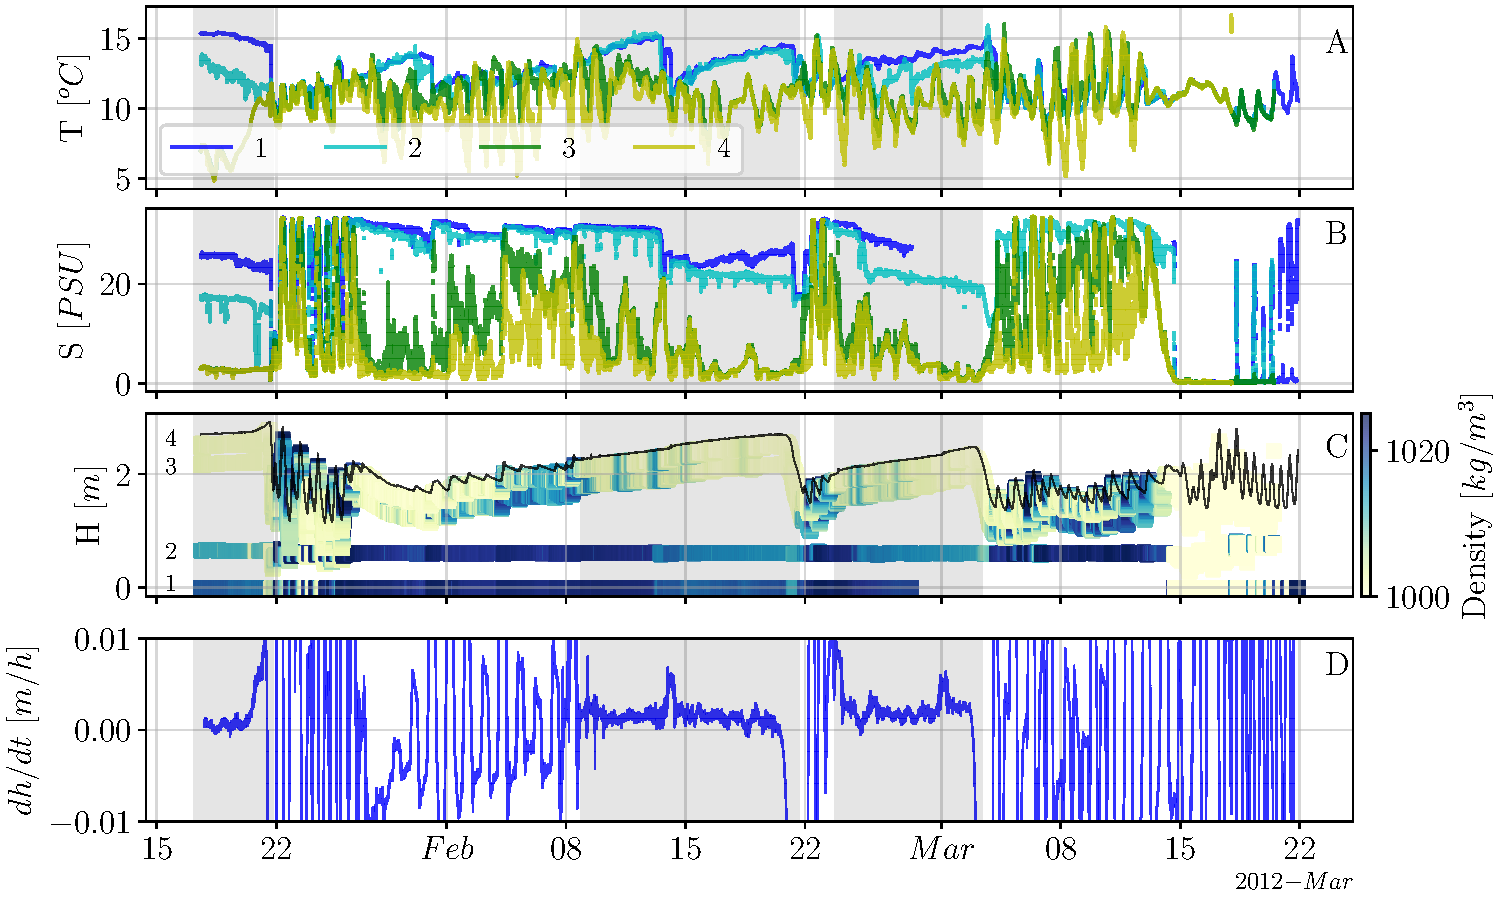
\includegraphics[scale=0.5]{Imagenes/saltemp.png}
    \caption{Time-series windowing at both closure phases of temperature and salinity in NM, where 1 is the deepest sensor and 4 the shallowest, colormap of density in NM in the water column, where the black line represents the water level, and the change of the water level in a 10-hour frame.}
    \label{fig:saltemp}
\end{figure}

We defined closed state at the estuary when the depth's change in time $\Delta h/\Delta t$, with $\Delta t=10$ hours, is positive and less than 0.01 m/h for more than a day (Fig. \ref{fig:saltemp}), meaning that the lagoon is filling with freshwater, increasing its level, and with a low influence from the sea. In that context Pescadero is in closed state three times, in mid January, in mid February, and in late February/early March where the first is at the start of the time series, not including the initial closure, while the second and third are in gray shadow (Fig. \ref{fig:saltemp}). The differences between these three closures are that the first has the highest water level, and second and third closures never get to the same level. \\

In the time series we observed during closed state the temperature and salinity went stratified (Fig. \ref{fig:saltemp}). We observed a lower and non stable temperature at the surface (Sensors 3 and 4 in Fig. \ref{fig:saltemp}) due to the cold season and the following of day-night temperature changes. The temperature at the bottom (Sensors 1 and 2 in Fig. \ref{fig:saltemp}) is more stable, but still being influenced by daily changes and other external factors, indicating for example an abrupt fall on February 13th, and then started to increase again. The bottom salinity is also steady most of the time and is generally decreasing. The surface salinity is more vulnerable to external factors, and only is more stable during closed state. \\ 

During closed state, we observed three layers in the density structure with the superior one getting thicker upstream. In Fig. \ref{fig:perfiles1} there is the longitudinal view of the estuary densities from the profiles and the moorings. We can observe that in near the mouth the salinity is higher or the water column is more homogeneous. After a few days in closed state, the estuary opened on February 21st and March 3rd observing a decrease in water level. \\

\begin{figure}[h!]
    \centering
    \includegraphics[scale=0.6]{Imagenes/vista_long2.png}
    \caption{Along-estuary density colormap of Pescadero. Distance x is considered from the coast following the curvature of the estuary as the sensors are placed in Fig. \ref{fig:mapPDO}. }
    \label{fig:perfiles1}
\end{figure}

\subsubsection{Tidal and waves conditions}

In Fig. \ref{fig:wave1} we have the wave conditions for Pescadero during the study period. We can observe, that when the mouth is open tidal influence is present in Pescadero, but when the mouth closes we cannot observe an evident effect at plain sight, which does not mean there is not present. Significant wave height goes from 2.5 m to more than 5 m approximately, but we have to account that deep water wave heights are larger than wave heights experienced at the coast (\cite{Williams2014}), and as this data where collected 40 km from shore, thus we use this value as a proxy for coastal ocean conditions.  \\

The rest of the parameters (wave periods and direction) were collected for the same buoy, so they also are an approximation of the wave conditions. Dominant periods go from 5 to 20 s, while averaged periods have al range only between 7 and 10 s. Direction of the dominant period is stable around the 300 degrees most of the time, with just a peak on February 29th where reaches the 250 degrees.\\

\begin{figure}[h!]
    \centering
    \includegraphics[width=\textwidth]{Imagenes/wave1.png}
    \caption{Time-series of tidal height in San Francisco (blue) and Pescadero estuary water level (black) in MLLW datum, significant wave height ($H_{SW}$), dominant wave period ($T_{DW}$), average wave period ($T_{AW}$) and the direction from which the waves at the dominant period are coming ($dir_{DW}$).}
    \label{fig:wave1}
\end{figure}

\subsubsection{Pescadero creek discharge}

Pescadero estuary receives freshwater from Butano Creek and Pescadero Creek, where the latter is the one that contributes the most to the lagoon and the one we have available data. When the inlet is closed, the maximum flow recorded was $0.72 m^3/s$, lower than the usual for winters in California, presenting two small increases in flow (Fig. \ref{fig:q}), but which, due to their low magnitude, would not be a determining factor in the rupture, considering that between July 2011 and July 2012 the maximum flow was $29.73 m^3/s$. Even so, there is a constant inflow of fresh water that increase the estuary water level progressively until the inlet breaks.  

\begin{figure}[h!]
    \centering
    \includegraphics[width=\textwidth]{Imagenes/Q.png}
    \caption{Time-series of freshwater flow from Pescadero Creek.}
    \label{fig:q}
\end{figure}

\subsubsection{Currents speed and direction}

During closed state, the wind direction is predominantly onshore and its magnitude in that direction is bigger than in the rest of the period (See Figs. \ref{fig:windvel} and \ref{fig:vels}). Surface wind stress over the closed estuary causes the upper layer to go in the same direction as the wind, and the lower layer to move in the opposite direction. Given the limitations of the ADCP sensor, velocities near the surface were not always captured, therefore, we observed a range of speed, not showing what happens at the bottom or the surface. \\

Fig. \ref{fig:vels} shows that as the wind increases, the along-estuary speeds ($u$) increase in a similar proportion, but in opposite direction. Wind is also influencing cross-estuary velocity ($v$), but in less intensity. Vertical velocity ($w$) present fluctuations and some negative or positive peaks during wind events or after in some cases. 

% Pescadero has its main directions very mrked, case that is very prticular in this jkind of estuaries, where along-estuary velocities always domain the currents (local forcing)

\begin{figure}[h!]
    \centering
    \includegraphics[width=\textwidth]{Imagenes/vels.png}
    \caption{Time-series of $u$ and $v$ in the water column, averaged vertical velocity, and wind stress.}
    \label{fig:vels}
\end{figure}

\subsubsection{Surface fluctuations}

We can observe, that when the mouth is open tidal influence is present in Pescadero, and when significant wave height increases the influence is also larger (Fig. \ref{fig:wave1}). When the bar blocks the inlet, this causes accumulation of the upstream freshwater in the lagoon which is represented as an increase in Pescadero water level, reducing the ocean influence to be negligible to plain sight, but still could be wave overtopping. This wave overtopping can be detected by the fluctuations in the surface present in the data, but also we have to consider the fluctuations caused by wind stress or by an increment of the discharge.\\

\subsection{Stratification controllers}

The external factors that could be affecting the estuary in closed state are freshwater inflow, saltwater intrusion, and wind stress. There are other factors involved as temperature or evaporation, but we estimated that those were negligible due to the haline stratification that dominates the estuary structure.

It is known that the first breach of the bar was artificial (Williams, 2014), openings that according to Behrens et al. (2013) would be less effective in keeping the mouth open than those that developed naturally, as in this case where the estuary is in open state for just a couple days. The second barrier breach is believed to have occurred naturally. 

We can notice a wind event in the offshore direction just before there is an increase in the Pescadero creek discharge, and we can observe this situation before other increases in flow, meaning the change of direction of the wind could happen during a storm.

\subsubsection{Wind stress}

At the beginning of both periods of disconnection, we noticed that there were changes in densities on the surface and in the deep layer, although the latter in smaller magnitude and fewer times (Figure 4). Three important wind events occurred in each period that matches with the increase in surface densities, observing that when the stress on the surface increases, so does the density in the upper layer in the three sensors. When wind forcing decreases, we noticed that density tends to return to its initial state, except for the largest events at the beginning of both periods, where density at the bottom is smaller after the event than before.

\begin{figure}[h!]
    \centering
    \includegraphics[width=\textwidth]{Imagenes/dens.png}
    \caption{Time-series of wind stress, NM, ML and DC densities in different depths, where the sensor 1 is the deepest and the sensor 4 is the shallowest (The positions in the water column of the sensors are showed in Fig. \ref{fig:perfiles1}), significant wave height in Halfmoon Bay (blue), Pescadero estuary water level (black) and tidal height in San Francisco (gray) in MLLW datum, and freshwater inflow of Pescadero creek.}
    \label{fig:dens}
\end{figure}


Upstream inflow had two increasing events in the studied period (Figure 4) and during those events, there wasn't an instant change in density, but we can notice that there is a trend in density, especially in the lower layers, where density is decreasing in time in both disconnected periods in NM and ML. In the first period, at DC location, different to the others, there is an increasing trend of density, which would not be unusual considering the lower layer of DC is much deeper than the ones of NM and ML (Figure 3), and the layer in DC with the same depth to those is the one before the deeper (in cyan, Figure 4-B). Another change in density that is noticeable occur in the middle layer of NM (in green, Figure 4-D) between February 13th and 17th, just before and after there was an increase in discharge, where density started being around 1015 kg/m3 and ended at almost 1000 kg/m3. 

%%Hablar de las olas en el periodo de la boca abierta
On the other hand, we could point out wave overtopping events in the estuary with wavelet analysis of the water level of the estuary (Figure 4-F), which identifies changes in its fluctuations showing when there is the presence of certain frequencies that could represent the ocean influence, crossed with tidal behavior and significant wave height. In Figure 4 we can observe increases in these frequencies' occurrence at the same time there are high waves and tide most of the time, but sometimes the wavelet analysis captures a signal during high tide but low wave height.

Wave overtopping does not represent an important presence on density data, so we do not have too much saltwater intrusion, however, there are small changes in density both on the bottom and on the surface. On March 1st we observed a salt intrusion event with no wind stress on the surface, evidencing density fluctuations in locations NM, ML, and DC, but without causing important density changes (Figure 4), also we observed something similar on February 14th, 19th and 26th but right after the wind event, so we can't know which factor is causing it. On February 15th we observed after wave overtopping that there was an increase in salinity at NM bottom that doesn't look like the increases in salinity caused by wind effects, because the salinity is bigger than the one before the wind event. Although, as this still happens when there was a wind event, we can't attribute it just to salt intrusion. Between February 25th and 28th, there are three salinity increases at NM bottom happening at the same time there is high tide and where the last one is observable in ML too. Even though wave overtopping in these points is not too noticeable in wavelet analysis and those events happened after three different wind events it could be an influence in density due to salt intrusion in the estuary that contributes to wind influence. 

%% graficar lo mismo que antes pero en vez de densidades con la superficie

\begin{figure}[h!]
    \centering
    \includegraphics[width=\textwidth]{Imagenes/dens.png}
    \caption{Time-series of wind stress, NM, ML and DC densities in different depths, where the sensor 1 is the deepest and the sensor 4 is the shallowest (The positions in the water column of the sensors are showed in Fig. \ref{fig:perfiles1}), significant wave height in Halfmoon Bay (blue), Pescadero estuary water level (black) and tidal height in San Francisco (gray) in MLLW datum, and freshwater inflow of Pescadero creek.}
    \label{fig:dens}
\end{figure}

\subsection{Wind-driven effects}

As mentioned before, we noticed changes in density at the same time there were wind events, therefore for quantifying those events we calculated the potential energy anomaly of the water column in location NM and compared it to wind stress (Figure 5), where we noticed that there were a lot of similarities between both time-series. We observed that when wind stress magnitude increases, potential energy anomaly decreases, except when there are positive values like on February 28th and 29th, when there was no change in potential energy anomaly. However, we can notice that the potential energy anomaly has not the same behavior in two wind events of the same magnitude, and we can observe that, in time, wind decreases its effect on the potential energy anomaly, only reaching 0 at the firsts wind events of each period, in addition, we can observe that after those events there is a decrease in potential energy anomaly when wind stress is zero, showing a change in their stratification structure after those events.

%% imagen potential anomaly wind stress 

For further understanding, we implemented the Wedderburn number to observe if there was upwelling due to wind events. As we did not have the thickness of the epilimnion we estimated a range of positions for the pycnocline. This range started right after the first CTD, the deeper one (in black), and ended in the second CTD (in grey) (Figure 6-D). As we are working with a range of values, we considered a partial upwelling when just the upper boundary reaches W=1 and full upwelling when both boundaries reach that value. In each period we noticed one full upwelling event and two partial upwelling events, for a total of six upwelling events, always the first one being fully upwelled (Figure 6). After full upwelling events, density at the bottom of the water column did not come back to its original values from before the event. 

%% imagen de esfuerzo de viento, densidad en nm, W y densidad en NM vertical

In Figure 6 we can observe how density at the surface is getting more resilient to wind effects in time. The three wind events in the first period are similar in magnitude, but the increase in density that they make is each time smaller, even though we can notice a small increase in wind stress at the beginning of the time series that increase density three times more than the last wind event in the period. We can also notice that with the density changes in the vertical where at the first wind events of both periods reached 0 but after those started going steadier.

The first important wind event started on February 13th at 2 a.m. and the first location that was affected was NM, then ML, and finally DC. We can prove that with the change of density along the estuary (Figure 7-C) where we observed negative values almost all the time, showing there are higher values in NM than in DC. When the wind starts to blow there is an increase of $\Delta \rho/\Delta x$ magnitude, and after reaching the peak the value decreases again to zero and stays there if the wind speed is constant. If wind speed decreases there is another increase in $\Delta \rho/\Delta x$ magnitude, showing that the wind stops influencing DC location first and then NM.

%imagen de wind stress,densidad superficial, cambios de densidad en la horizontal y en la vertical

To quantify the time difference between the moment wind started blowing and density started changing at the different CTD locations, we calculate by visual inspection how long it took for the wind to affect density at different points. To achieve this, we considered the moment that density just started to change into a trend after the wind started or stopped blowing. Also, to compare the obtained values we calculated the cross-correlation, between density and wind stress, first normalizing and standardizing both signals. We obtained the values of only the first wind event, how long took to start, and end, and for the cross-correlation we added the total of the first-period lag.

In Table 1 we observed that surface sensors (NM3, DC4, and ML2) had no delay with the cross-correlation method and did have it with a visual inspection. Also, at the latter, we observed that NM3 was the last sensor that started to change after wind stress started, but it increased faster than the others, fact that we can observe slightly in Figure 7-B. Also, we observed that the one that took longer to come back to its initial value was NM3, then ML2 and DC4.

\subsubsection{Upwelling and circulation}

\subsubsection{Dynamic response}



\section{Discussion}

\textit{Para mí el capitulo fundamental. Los resultados son analizados en detalle, pudiendo incorporar análisis adicionales que no estaban inicialmente en la metodología, como para entender, entre otras cosas, la sensibilidad de los resultados ante parámetros por ejemplo. O la comparación con resultados de otros estudios, o conocimiento existente. En este capítulo se debe entender si lo que se hizo es útil o no.}

Near the mouth the upper layer is thinner probably because the salinity is higher due to the waves that are overtopping the sandbar.

Pescadero funciona como tal y tales cuerpos de agua (buscar) (discusion de kelly 2017 buena)
payandeh tiene algunos pára comparar con enfoqye de viento
wind: orientation of the bay, shallowness

colocar problemas de los métodos de analisis
wedberner number is too aproximasted
frequency analysis doesnt show an specific time, shows all the dataset

acording to Paugam 2021 the drag coefficient Cd can be difficult to estimate in shallow water %discusion?

\section{Conclusions}

\textit{1 o 2 páginas que resuman lo aprendido, y verifiquen que los objetivos se cumplieron.}

\subsection{Estructura (Utilizar este estilo de subtítulo dentro de cada sección)}
Utilizar la siguiente estructura para las secciones principales, como por ejemplo: Introducción, Objetivos, Metodología, Resultados, Discusión, Conclusiones y Referencias. Los títulos específicos de cada sección deben fijarse de acuerdo al tema de la memoria en conjunto con el profesor supervisor.\\

La memoria podrá tener una extensión de máximo 30 páginas, sin contar con la portada y hoja de firmas.


\printbibliography
\end{document}